The main text reports the AI-channel-attributable shortfall
($\sim$70{,}000 missing questions) using the DDD coefficient
applied cell by cell. For context, we describe in this
appendix the relationship between this DDD-implied
counterfactual and a simpler descriptive counterfactual
based on linear extrapolation of the pre-ChatGPT aggregate
trend.

\subsection{Linear extrapolation of the pre-ChatGPT trend}

The pre-ChatGPT log-linear regression of the weekly total
on time is
$\log Q_w = c + \rho w$ with $\hat\rho = -0.00333$ per week
and $R^2 = 0.80$. Extrapolating into the post-ChatGPT
window implies a counterfactual aggregate of $\sim$3.09
million questions; observed is $\sim$1.67 million; the
implied break from trend is $\sim$1.42 million questions
or $-46\%$ from the trend-implied path.
Figure~\ref{fig:counterfactual_app} shows the two
trajectories with the shaded shortfall area.

\begin{figure}[!htbp]
\centering
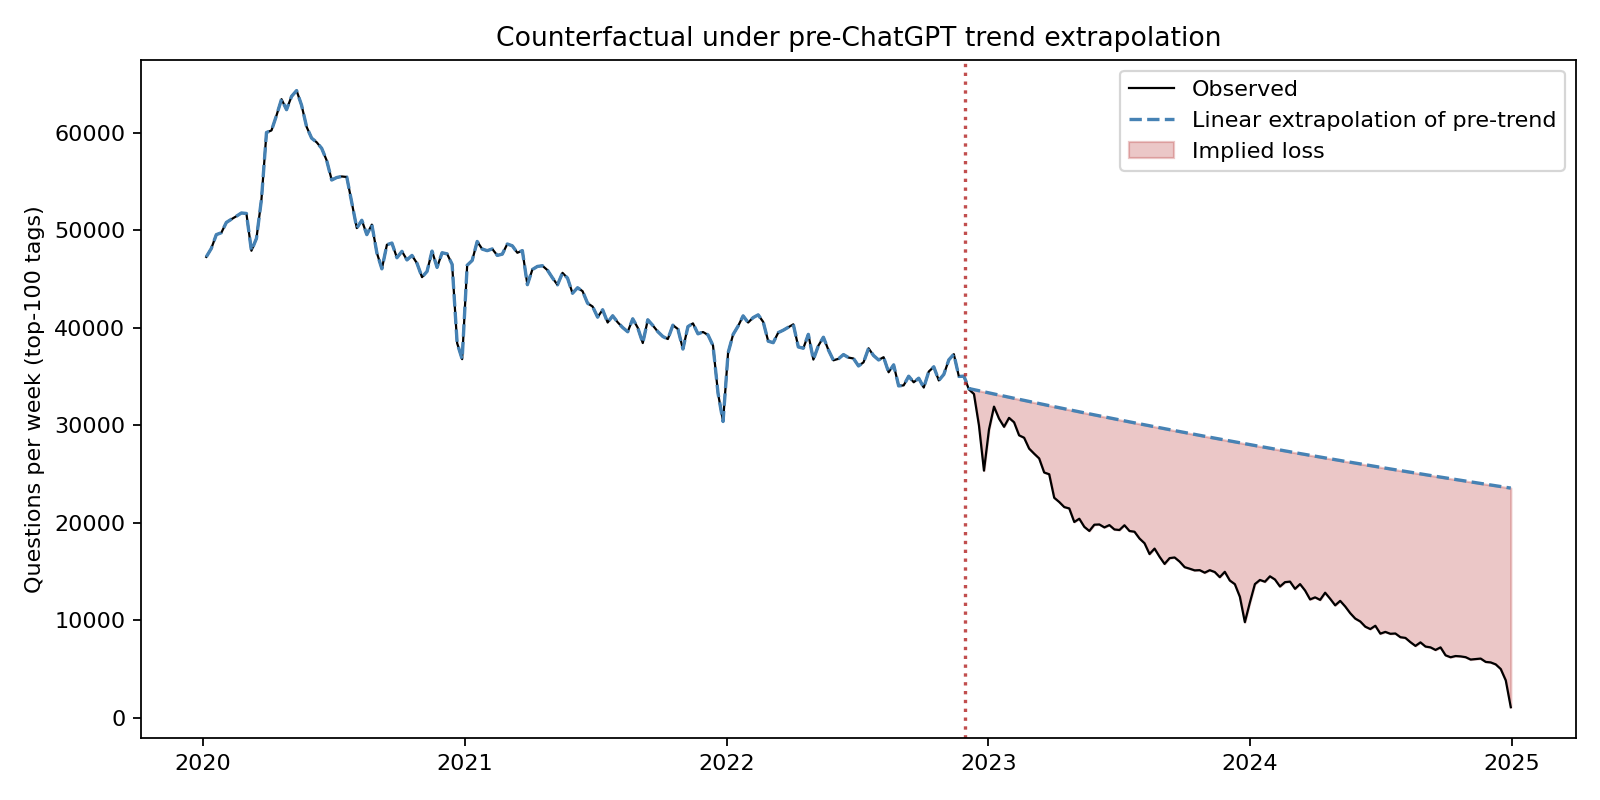
\includegraphics[width=0.92\textwidth]{figures/economic_magnitude_counterfactual.png}
\caption{Aggregate weekly questions observed vs.\ linear
extrapolation of pre-ChatGPT trend. Vertical line: ChatGPT
release. Shaded area: implied break from trend
(descriptive only, not causal).}
\label{fig:counterfactual_app}
\end{figure}

\subsection{Why this descriptive number is not the causal
effect}

The 1.42-million figure is \emph{descriptive only}. It
attributes the entire break from the pre-trend to the
ChatGPT release; this attribution is not justified by the
data, because the pre-treatment trend itself reflects a
mix of forces (maturation of the platform, secular shift to
private channels, prior LLM access via Codex and earlier
GPT releases). The DDD design corrects for this by
identifying a within-tag, within-question-type residual:
that residual corresponds to roughly $\sim$70{,}000
missing questions, not 1.42 million.

We retain the descriptive number in the appendix for two
reasons: (a) it provides a maximum-credible upper bound on
the size of the AI-mediated channel that the DDD is
narrowing within; and (b) it makes visible how much of the
post-ChatGPT decline is \emph{not} identified by our design
(approximately 96\%). The main paper uses the DDD-implied
counterfactual ($\sim$70{,}000) and explicitly states the
DDD's identification scope.
